\documentclass[10pt]{article}
\usepackage{amsmath,amssymb,amsthm,graphicx}
\usepackage[margin=1in]{geometry}
\usepackage[hidelinks]{hyperref}
\newtheorem{theorem}{Theorem}
\newtheorem{proposition}{Proposition}
\newtheorem{lemma}{Lemma}
\newcommand{\R}{\mathbb R}
\title{Assessment of Exact Polynomial Bellman Values}
\author{Research notes}
\date{23 October 2026}
\begin{document}
\maketitle

\section{Question and scope}

The question is whether the polynomial examples in \texttt{maximal\_element\_bellman.tex} support an exact finite conic solution for a class of interacting control systems. A sum of squares is a finite sum of squared polynomials. Polynomial Bellman lower bounds computed by sum of squares are established methods \cite[Section III]{summers}. The missing requirement is that the optimal value itself have the proposed polynomial form. This assessment tests that requirement for the coupled quartic example and for a larger parameterized class. It also examines persistence under perturbations and the proposed use of polynomial lifts. No publication priority is claimed for the results proved here.

A polynomial is homogeneous of degree $d$ if every nonzero monomial has total degree $d$. A quartic has degree four.

\section{A coupled control problem}

Fix
\begin{equation}
 \alpha,\beta,q_1,q_2,\rho>0,\qquad \eta\geq0,\qquad 0<\gamma\leq1.
 \label{eq:data}
\end{equation}
For $x=(s,t)\in\R^2$ and $u\in\R$, define the successor and stage cost by
\begin{equation}
 F(s,t,u)=(\alpha t,-\beta s+u),\qquad
 \ell_\eta(s,t,u)=q_1s^4+q_2t^4+\eta s^2t^2+\rho u^4.
 \label{eq:problem}
\end{equation}
Let $J_\eta(x)$ be the infimum of $\sum_{k=0}^\infty\gamma^k\ell_\eta(x_k,u_k)$ over all control sequences, with $x_0=x$ and $x_{k+1}=F(x_k,u_k)$. Controls are unrestricted. The feedback $u=\beta s$ gives successive states $(\alpha t,0)$ and $0$. Its cost is
\begin{equation}
 D_\eta(s,t)=(q_1+\rho\beta^4)s^4+
 \bigl[q_2+\gamma\alpha^4(q_1+\rho\beta^4)\bigr]t^4+\eta s^2t^2.
 \label{eq:deadbeat}
\end{equation}
The first stage cost and this admissible feedback give
\begin{equation}
 q_1s^4+q_2t^4+\eta s^2t^2\leq J_\eta(s,t)\leq D_\eta(s,t).
 \label{eq:bounds}
\end{equation}
In particular, the value is finite everywhere.

\begin{lemma}
\label{lem:symmetry}
The value satisfies
\begin{equation}
 J_\eta(rs,rt)=r^4J_\eta(s,t),\qquad
 J_\eta(\epsilon_1s,\epsilon_2t)=J_\eta(s,t)
 \quad(r\geq0,\ \epsilon_1,\epsilon_2\in\{-1,1\}),
 \label{eq:symmetry}
\end{equation}
and the Bellman equation
\begin{equation}
 J_\eta(s,t)=q_1s^4+q_2t^4+\eta s^2t^2+
 \inf_{u\in\R}\{\rho u^4+\gamma J_\eta(\alpha t,u-\beta s)\}.
 \label{eq:bellman}
\end{equation}
\end{lemma}
\begin{proof}
For $r>0$, multiplying every state and control of a trajectory by $r$ gives a bijection between trajectories from $x$ and $rx$. Equation~\eqref{eq:problem} multiplies every stage cost by $r^4$. Taking infima proves the first equality in \eqref{eq:symmetry}. At $r=0$, the zero trajectory and nonnegative costs give the equality.

For signs $\epsilon_1,\epsilon_2$, write $E=\operatorname{diag}(\epsilon_1,\epsilon_2)$ and $E'=\operatorname{diag}(\epsilon_2,\epsilon_1)$. Direct substitution gives
\[
 F(Ex,\epsilon_1u)=E'F(x,u),\qquad
 \ell_\eta(Ex,\epsilon_1u)=\ell_\eta(x,u).
\]
Alternate $E$ and $E'$ along the trajectory and multiply each control by the current first sign. This operation is its own inverse and preserves total cost, proving the second equality in \eqref{eq:symmetry}.

Splitting any trajectory after its first action gives the lower inequality in \eqref{eq:bellman}. Conversely, for any first action, append a trajectory whose cost is within any prescribed positive tolerance of the finite successor value. Take the infimum over the first action and let the tolerance tend to zero. This proves the reverse inequality.
\end{proof}

\begin{theorem}
If $\eta>0$, then $J_\eta$ is not a polynomial of any finite degree.
\label{thm:obstruction}
\end{theorem}
\begin{proof}
Suppose $J_\eta$ is polynomial. The scaling and sign identities in \eqref{eq:symmetry} remove every monomial except the three even monomials of degree four. Thus
\begin{equation}
 J_\eta(s,t)=a s^4+b s^2t^2+c t^4,
 \qquad a\geq q_1>0,\quad c\geq q_2>0,
 \label{eq:assumed}
\end{equation}
where the inequalities follow from \eqref{eq:bounds} on the coordinate axes. The objective in \eqref{eq:bellman} is continuous and at least $\rho u^4$, so it attains its minimum.

Define the polynomial residual
\begin{equation}
 R(s,t,u)=\ell_\eta(s,t,u)+\gamma J_\eta(\alpha t,u-\beta s)-J_\eta(s,t).
 \label{eq:residual}
\end{equation}
Equation~\eqref{eq:bellman} gives $R\geq0$ everywhere. At a minimizing action $u_*$ for $(s,t)=(0,1)$, $R(0,1,u_*)=0$. Therefore both partial derivatives $R_s$ and $R_u$ vanish there. Using \eqref{eq:assumed} gives
\[
 0=-\beta\gamma(2b\alpha^2u_*+4cu_*^3),\qquad
 0=4\rho u_*^3+\gamma(2b\alpha^2u_*+4cu_*^3).
\]
Adding the first equality divided by $\beta$ to the second gives $u_*=0$. The second derivative with respect to $u$ at this minimum is $2\gamma b\alpha^2$, so $b\geq0$. Equation~\eqref{eq:bellman} at $(0,1)$ now gives
\begin{equation}
 c=q_2+\gamma\alpha^4a.
 \label{eq:axis-relation}
\end{equation}
Substitute \eqref{eq:assumed} and \eqref{eq:axis-relation} into \eqref{eq:bellman} at $(1,t)$. The result is
\begin{equation}
 a-q_1+(b-\eta)t^2=m(t),\qquad
 m(t)=\min_u\{\rho u^4+\gamma b\alpha^2t^2(u-\beta)^2
                         +\gamma c(u-\beta)^4\}.
 \label{eq:scalar-minimum}
\end{equation}
Every term in this minimum is nonnegative, and $u=\beta$ gives $m(t)\leq\rho\beta^4$. Boundedness for all $t$ forces $b=\eta$. Hence \eqref{eq:scalar-minimum} requires $m(t)$ to be constant.

The function $u\mapsto\rho u^4+\gamma c(u-\beta)^4$ has a strictly positive second derivative for every $u$, since $\beta>0$. Its unique minimizer is
\[
 u_0=\frac{(\gamma c)^{1/3}}{\rho^{1/3}+(\gamma c)^{1/3}}\,\beta,
 \qquad 0<u_0<\beta.
\]
For $t\ne0$, equality $m(t)=m(0)$ would require both $u=u_0$ and $u=\beta$, since the additional term in \eqref{eq:scalar-minimum} is nonnegative and $b=\eta>0$. These requirements are incompatible. The minimum is attained, so $m(t)>m(0)$ for $t\ne0$, contradicting constancy.
\end{proof}

The result applies to a controllable linear plant: its input column is $(0,1)^\top$, and that column together with its image $(\alpha,0)^\top$ has rank two. At $\alpha=\beta=1$, the uncontrolled dynamics are a quarter-turn rotation. At $q_1=q_2=1$ and $\eta=2$, the state cost is $(s^2+t^2)^2$. Thus the obstruction already occurs for an elementary linear oscillator with a convex quartic cost and one actuator.

\begin{proposition}
If $\eta>0$, no stationary feedback whose action is polynomial in $(s,t)$ is optimal at every state.
\label{prop:feedback}
\end{proposition}
\begin{proof}
For such a feedback $\mu$, optimality and \eqref{eq:bounds} imply
\[
 \rho|\mu(x)|^4\leq J_\eta(x)\leq C\|x\|_2^4
\]
for some $C<\infty$. Restricting a polynomial $\mu$ to every line through zero shows that its degree is at most one. The same inequality gives $\mu(0)=0$, so $\mu$ is linear.

Under a linear feedback, each partial cost is a homogeneous quartic in $(s,t)$, since the state and input at every time are linear in the initial state. Evaluate these partial costs at $(r,1)$ for five distinct real numbers $r$. Their values converge because the feedback has finite cost. The five coefficients are recovered by an invertible Vandermonde matrix, whose entries are the corresponding powers of $r$, so the coefficients also converge. The limiting cost is therefore a homogeneous quartic at every state. Optimality would make this polynomial equal to $J_\eta$, contrary to Theorem~\ref{thm:obstruction}.
\end{proof}

\section{The exact case with zero coupling}

For $v,w>0$, define
\begin{equation}
 h(v,w)=(v^{-1/3}+w^{-1/3})^{-3},\qquad h(v,0)=0.
 \label{eq:h}
\end{equation}
Differentiating $vu^4+w(u-z)^4$ shows that its minimum is $h(v,w)z^4$. Start $a_0=c_0=0$ and iterate
\begin{equation}
 a_{j+1}=q_1+\beta^4h(\rho,\gamma c_j),\qquad
 c_{j+1}=q_2+\gamma\alpha^4a_j.
 \label{eq:iteration}
\end{equation}
Both sequences increase: $h(v,w)$ increases with $w$, and the initial update is positive. Also $0\leq h(\rho,w)\leq\rho$, so
\[
 a_j\leq q_1+\rho\beta^4,\qquad
 c_j\leq q_2+\gamma\alpha^4(q_1+\rho\beta^4).
\]
They converge to positive limits $a_0^*,c_0^*$ satisfying the fixed point equations in \eqref{eq:iteration}. Define
\begin{equation}
 V_0(s,t)=a_0^*s^4+c_0^*t^4,\qquad
 k=\frac{(\gamma c_0^*)^{1/3}}{\rho^{1/3}+(\gamma c_0^*)^{1/3}},
 \qquad \mu_0(s,t)=k\beta s.
 \label{eq:baseline}
\end{equation}

\begin{proposition}
The value for $\eta=0$ is $J_0=V_0$, and $\mu_0$ is optimal. For every $\eta\geq0$, $V_0\leq J_\eta$, with equality on both coordinate axes.
\label{prop:baseline}
\end{proposition}
\begin{proof}
Equations~\eqref{eq:h}--\eqref{eq:baseline} give
\[
 V_0(x)\leq\ell_0(x,u)+\gamma V_0(F(x,u)),
\]
with equality under $\mu_0$. Multiplication by $\gamma^j$ and summation give
\begin{equation}
 V_0(x_0)-\gamma^NV_0(x_N)
 \leq\sum_{j=0}^{N-1}\gamma^j\ell_0(x_j,u_j),
 \label{eq:baseline-sum}
\end{equation}
again with equality under $\mu_0$. On any finite-cost trajectory,
\[
 \gamma^N\|x_N\|_2^4\leq
 \frac{2\gamma^N\ell_0(x_N,u_N)}{\min(q_1,q_2)}\longrightarrow0.
\]
Since $V_0(x)\leq C_0\|x\|_2^4$, passage to the limit in \eqref{eq:baseline-sum} gives $V_0\leq J_0$. Under $\mu_0$, equality in \eqref{eq:baseline-sum} and nonnegativity of the terminal value bound every partial cost by $V_0(x_0)$. The resulting finite cost makes the terminal term vanish, proving $J_0=V_0$. Increasing $\eta$ only increases trajectory costs, so $J_\eta\geq J_0$. Under $\mu_0$, a state on either coordinate axis remains on the union of the axes. The added term $\eta s^2t^2$ vanishes along that trajectory, proving equality on the axes.
\end{proof}

Together, Theorem~\ref{thm:obstruction} and Proposition~\ref{prop:baseline} characterize polynomiality for \eqref{eq:problem}: the value is polynomial exactly when $\eta=0$. The exact case separates into two alternating scalar control problems. It does not supply the sought extension to coupled polynomial values.

\section{What increasing the polynomial degree can accomplish}

Call a polynomial $W$ a normalized nonnegative Bellman subsolution if
\begin{equation}
 W(0)=0,\qquad W(x)\geq0,\qquad
 W(x)\leq\ell_\eta(x,u)+\gamma W(F(x,u))
 \quad(x\in\R^2,\ u\in\R).
 \label{eq:subsolution}
\end{equation}
Normalization is necessary when $\gamma=1$, since constant shifts otherwise preserve the Bellman inequality.

\begin{theorem}
\label{thm:degree}
Every polynomial satisfying \eqref{eq:subsolution} is homogeneous of degree four or identically zero, and is a lower bound on $J_\eta$. If $\eta>0$, there is $\varepsilon_*>0$ such that every such polynomial satisfies
\begin{equation}
 \sup_{\|x\|_2=1}|J_\eta(x)-W(x)|\geq\varepsilon_*.
 \label{eq:uniform-gap}
\end{equation}
\end{theorem}
\begin{proof}
Apply \eqref{eq:subsolution} twice along the trajectory used in \eqref{eq:deadbeat}:
\[
 W(s,t)\leq\ell_\eta(s,t,\beta s)
       +\gamma\ell_\eta(\alpha t,0,\beta\alpha t)+\gamma^2W(0)
       =D_\eta(s,t).
\]
Together with nonnegativity, this gives
\begin{equation}
 0\leq W(x)\leq D_\eta(x)\leq C\|x\|_2^4.
 \label{eq:polynomial-bound}
\end{equation}
For fixed $x$, the univariate polynomial $r\mapsto W(rx)$ is nonnegative and bounded above by $C\|x\|_2^4r^4$ for every $r>0$. Its largest nonzero power cannot exceed four, by letting $r\to\infty$. Its smallest nonzero power cannot be less than four, by letting $r\downarrow0$. Thus $W(rx)=r^4W(x)$. Applying this identity to every $x$ eliminates all terms of degrees other than four.

For any finite-cost trajectory, the tail estimate in the proof of Proposition~\ref{prop:baseline} applies because $\ell_\eta\geq\ell_0$. Equation~\eqref{eq:polynomial-bound} then makes $\gamma^NW(x_N)\to0$. Summing \eqref{eq:subsolution} gives
\[
 W(x_0)-\gamma^NW(x_N)\leq
 \sum_{j=0}^{N-1}\gamma^j\ell_\eta(x_j,u_j).
\]
Passage to the limit gives the lower bound for finite costs; infinite costs satisfy the same bound. Hence $W\leq J_\eta$.

If \eqref{eq:uniform-gap} failed, there would be homogeneous quartics $W_j$ converging uniformly to $J_\eta$ on the unit circle. Evaluate them at the five normalized points $(r,1)/\sqrt{1+r^2}$ with $r=-2,-1,0,1,2$. Multiplication of these values by $(1+r^2)^2$ gives an invertible Vandermonde system for the five coefficients. Uniform convergence therefore makes all coefficients converge. The limiting polynomial equals $J_\eta$ on the circle and, by \eqref{eq:symmetry}, everywhere. This contradicts Theorem~\ref{thm:obstruction}.
\end{proof}

This conclusion concerns global nonnegativity and global Bellman inequalities on the unbounded state domain. It does not concern polynomial approximation restricted to a compact domain or representations that use several polynomial pieces. Even allowing arbitrary polynomial degree in \eqref{eq:subsolution} cannot close the uniform gap.

The degree argument has a wider scope. For any integer $d\geq1$, a polynomial satisfying $0\leq W(x)\leq C\|x\|_2^d$ everywhere is either zero or homogeneous of degree $d$: the limits along rays used in the proof of Theorem~\ref{thm:degree} eliminate all other powers. Thus globally nonnegative polynomial lower bounds on any value satisfying that growth bound have the same restriction. Both the behavior near zero and the behavior at infinity are needed for this conclusion.

At quartic degree, a further source of conservatism is absent in this example. The residual in \eqref{eq:subsolution} is a homogeneous quartic in the three variables $(s,t,u)$. Hilbert's theorem states that every nonnegative homogeneous quartic in three variables is a sum of squares of quadratic polynomials \cite{powers}. Nonnegativity of $W$ has the same certificate, by treating it as independent of a third variable. A semidefinite program optimizes a linear function subject to affine equations and positive semidefinite matrix constraints. To describe \eqref{eq:subsolution}, write the residual as $z^\top Qz$ with $Q\succeq0$ and $z=(s^2,st,t^2,su,tu,u^2)^\top$, and write $W$ in the same way using $(s^2,st,t^2)^\top$. Matching coefficients gives affine equations in the entries of the positive semidefinite matrices and the coefficients of $W$. These constraints describe the entire set in \eqref{eq:subsolution}; the optimal value function remains outside that set.

A weighted sum of monomial coefficients need not define a positive integral objective. For
\[
 W(s,t)=p_1s^4+p_2s^3t+p_3s^2t^2+p_4st^3+p_5t^4,
\]
integration over the unit disk gives
\begin{equation}
 \int_{s^2+t^2\leq1}W(s,t)\,ds\,dt
 =\frac{\pi}{24}(3p_1+p_3+3p_5).
 \label{eq:moment-objective}
\end{equation}
The mixed odd powers integrate to zero. This is the appropriate objective for the disk; arbitrary positive weights on all five coefficients have no such general interpretation.

\section{Persistence under perturbations}

Fix the data in \eqref{eq:data} with $\eta>0$. Consider other two-state, one-input systems with linear dynamics $x^+=Ax+Bu$ and a homogeneous quartic stage cost $f(x,u)$. Closeness of these data means closeness of the entries of $A,B$ and of all monomial coefficients of $f$ to those in \eqref{eq:problem}.

\begin{theorem}
With $\gamma$ fixed, all sufficiently close data have a finite value everywhere, and that value is not a polynomial.
\label{thm:perturbation}
\end{theorem}
\begin{proof}
Use the fixed gain $K=(\beta,0)$. At the unperturbed data its closed-loop matrix is
\[
 M_0=\begin{bmatrix}0&\alpha\\0&0\end{bmatrix},\qquad M_0^2=0.
\]
Set $P=I+M_0^\top M_0$. Then $M_0^\top PM_0=P-I$. For every sufficiently close $M=A+BK$, continuity gives
\[
 M^\top PM\leq P-\tfrac12I
 \leq\left(1-\frac{1}{2\lambda_{\max}(P)}\right)P.
\]
Iterating this inequality bounds $\|M^jx\|_2$ by $H r^j\|x\|_2$, where $H<\infty$ and $r<1$ can be chosen uniformly in a neighborhood. The original cost is strictly positive on the unit sphere in $(x,u)$. Compactness of that sphere and coefficient continuity give uniform constants $e,E>0$ such that
\[
 e(\|x\|_2^4+|u|^4)\leq f(x,u)
 \leq E(\|x\|_2^4+|u|^4).
\]
The fixed feedback therefore has cost at most
\[
 E(1+\|K\|_2^4)H^4\sum_{j=0}^\infty\gamma^jr^{4j}\|x\|_2^4.
\]
Consequently all nearby optimal values lie between $e\|x\|_2^4$ and $C\|x\|_2^4$, with a uniform finite $C$.

Suppose there were polynomial values $V_j$ for a sequence of data converging to the original data. Homogeneity makes every $V_j$ quartic. The uniform bounds and the five evaluation points used in the proof of Theorem~\ref{thm:degree} bound all five coefficients. Select a subsequence whose coefficients converge to those of a quartic $V$. Then
\[
 e\|x\|_2^4\leq V(x)\leq C\|x\|_2^4.
\]
Every $V_j$ satisfies its Bellman equation. At a minimizing action, the control-cost lower bound gives $e|u|^4\leq V_j(x)\leq C\|x\|_2^4$. For fixed $x$, all minimizers thus belong to one compact interval. The objectives converge uniformly on that interval, because their polynomial coefficients and the plant entries converge. Taking the limit in their minima gives
\[
 V(x)=\min_u\{\ell_\eta(x,u)+\gamma V(F(x,u))\}.
\]
The minimum is attained. Summing the resulting Bellman inequality on finite-cost trajectories gives $V\leq J_\eta$, since $V(x)\leq C\|x\|_2^4$ makes the terminal term vanish. Choosing a minimizing action at every state bounds all partial costs by $V(x_0)$. These costs are finite, their terminal term also vanishes, and equality gives $J_\eta\leq V$. This contradicts Theorem~\ref{thm:obstruction}.
\end{proof}

The neighborhood in Theorem~\ref{thm:perturbation} permits general small changes to both plant matrices and all quartic cost coefficients. Individual sign symmetry is not required for the perturbed systems. The proof establishes existence of a neighborhood; it does not compute its radius.

The argument of Proposition~\ref{prop:feedback} also applies throughout this neighborhood. A polynomial optimal feedback would have at most linear growth and hence be linear; its finite cost would then be quartic. Thus the perturbed problems also have no globally optimal polynomial stationary feedback.

\section{A limitation of finite linear lifts}

Finite lifts are also an established control approach \cite{brunton}. An exact lift with unchanged inputs would require an identity of the form
\begin{equation}
 \Phi(Ax+Bu)=L\Phi(x)+Du
 \quad(x\in\R^n,\ u\in\R^m),
 \label{eq:lift}
\end{equation}
where $\Phi:\R^n\to\R^r$ is a chosen finite vector of functions and $L,D$ are constant matrices of compatible sizes.

\begin{proposition}
If $[A^{n-1}B\ \cdots\ B]$ has rank $n$, every $\Phi$ satisfying \eqref{eq:lift} is affine.
\label{prop:lift}
\end{proposition}
\begin{proof}
Start from $x_0=0$ and stack $n$ inputs into a vector $U$. Write
\[
 C_n=[A^{n-1}B\ \cdots\ B],\qquad
 D_n=[L^{n-1}D\ \cdots\ D].
\]
Iterating \eqref{eq:lift} gives $\Phi(C_nU)=L^n\Phi(0)+D_nU$. Rank $n$ provides a right inverse $C_n^\dagger$ with $C_nC_n^\dagger=I$. Choose $U=C_n^\dagger x$ to obtain
\[
 \Phi(x)=L^n\Phi(0)+D_nC_n^\dagger x.
\]
This is affine in $x$.
\end{proof}

This elementary observation concerns controllable linear plants, unrestricted inputs, and the constant-input-matrix identity \eqref{eq:lift}. It does not exclude bilinear lifts, input transformations, or useful exact lifts of specially structured nonlinear plants. It does show that a nonlinear polynomial lift cannot turn \eqref{eq:problem} into a new exact linear control problem with unchanged inputs.

For the separate nonlinear example in the original notes, the identity $x_1^+=a x_1+u$ gives
\[
 (x_1^+)^2=a^2x_1^2+2ax_1u+u^2.
\]
The proposed coordinate $x_1^2$ therefore already introduces state-dependent and quadratic input terms. Merely observing that the Bellman residual is polynomial does not prove finite linear closure or exactness of a conic value computation. Brunton and coauthors explicitly discuss input-induced limitations of finite lifts \cite[Section 5.2]{brunton}.

\section{Numerical check with controlled optimization and tail errors}

Set $\alpha=\beta=q_1=q_2=\rho=1$ and $\gamma=0.9$. The limits in \eqref{eq:baseline} satisfy
\begin{equation}
 a_0^*=1+k^3,\quad c_0^*=1+\gamma a_0^*,\quad
 k^3\bigl[(1-k)^{-3}-\gamma^2\bigr]=\gamma(1+\gamma).
 \label{eq:numerical-base}
\end{equation}
Numerically $k\simeq0.5509$, $a_0^*\simeq1.1672$, and $c_0^*\simeq2.0505$. Put $d=1-k$. Under $\mu_0$, the closed-loop matrix has square $-dI$, and the product of squared state components is multiplied by $d^2$ each step. The exact cost of this feedback for arbitrary $\eta\geq0$ is therefore
\begin{equation}
 V_K(s,t)=V_0(s,t)+\frac{\eta}{1-\gamma d^2}s^2t^2.
 \label{eq:upper}
\end{equation}
Proposition~\ref{prop:baseline} and admissibility give $V_0\leq J_\eta\leq V_K$.

The file \texttt{assess\_polynomial\_exactness.m} solves an 18-stage problem with terminal cost $V_0$, for $\eta=0,0.2,2$ and 15 state ratios. The objective is convex: its state-cost Hessian has nonnegative diagonal entries and determinant
\[
 24\eta(s^4+t^4)+(144-12\eta^2)s^2t^2\geq0
 \quad(0\leq\eta\leq2).
\]
The input fourth powers and terminal cost are also convex. With scaled states $\xi_j=\gamma^{j/4}x_j$ and inputs $v_j=\gamma^{j/4}u_j$, all discount factors disappear from the objective and the dynamics become $\xi_{j+1}=\gamma^{1/4}(A\xi_j+Bv_j)$. Let $L_N(v;x)$ denote this objective and let $g$ be its gradient at a computed input vector $v$. Its minimum is a lower bound on $J_\eta(x)$.

At an exact minimizer $v^*$, nonnegativity of every term and the feasible upper bound $V_K(x)$ imply $|v_j^*|\leq R_x$, where $R_x=V_K(x)^{1/4}$. The convex first-order inequality gives
\begin{equation}
 L_N(v;x)-\sum_{j=0}^{N-1}|g_j|(R_x+|v_j|)
 \leq \min_z L_N(z;x)\leq J_\eta(x)
 \leq L_N(v;x)+(V_K-V_0)(\xi_N).
 \label{eq:numerical-bounds}
\end{equation}
The last inequality appends $\mu_0$ to the computed finite trajectory. Thus the interval accounts for both incomplete numerical optimization and the infinite tail.

For $st\ne0$, define the effective mixed coefficient by
\begin{equation}
 b_{\rm eff}(s,t)=\frac{J_\eta(s,t)-a_0^*s^4-c_0^*t^4}{s^2t^2}.
 \label{eq:effective}
\end{equation}
A polynomial value satisfying the symmetry and axis values would require this quantity to be constant. The numerical states are $(1,r)/\sqrt{1+r^2}$, and the coupling coefficient is $\eta=2$.

\begin{table}[ht]
\centering
\caption{Bounds evaluated in floating point. The final column bounds the value uncertainty, not the uncertainty of the mixed coefficient.}
\label{tab:numerics}
\begin{tabular}{rrrr}
\hline
$r$ & Lower $b_{\rm eff}$ & Upper $b_{\rm eff}$ & Value interval width\\
\hline
0.1 & 2.366230 & 2.368218 & 1.95e-05 \\
0.3 & 2.382833 & 2.383125 & 2.21e-05 \\
1.0 & 2.280206 & 2.280351 & 3.64e-05 \\
3.0 & 2.074611 & 2.074644 & 2.89e-06 \\
10.0 & 2.006986 & 2.008145 & 1.14e-05 \\
\hline

\end{tabular}
\end{table}

The intervals in Table~\ref{tab:numerics} show that the variation in \eqref{eq:effective} exceeds the evaluated optimization and tail errors.

\begin{figure}[ht]
\centering
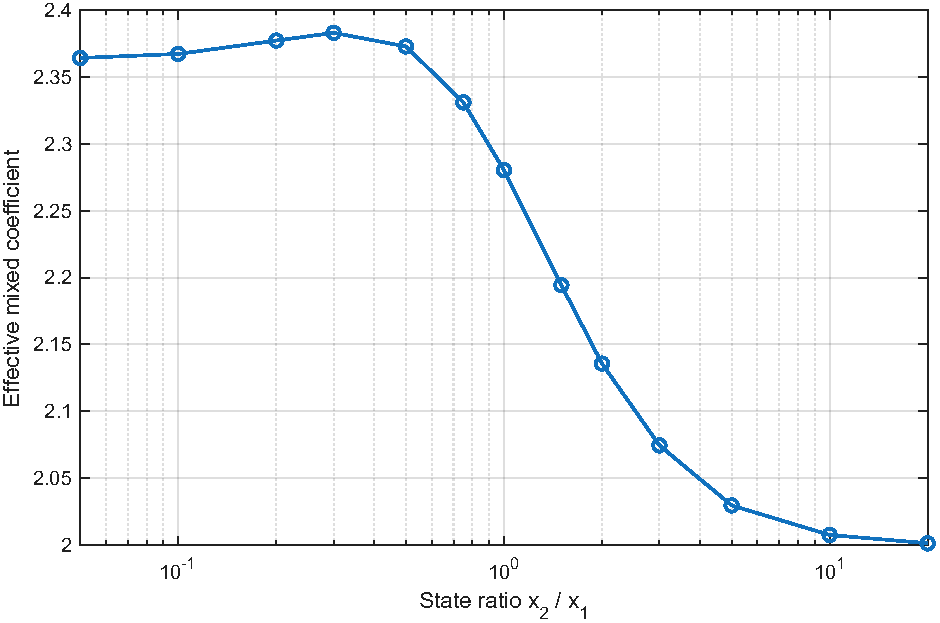
\includegraphics[width=.68\textwidth]{polynomial_results/mixed_coefficient.pdf}
\caption{Variation of the effective mixed coefficient for $\eta=2$. Points use midpoints of the evaluated bounds.}
\label{fig:mixed}
\end{figure}

The maximum value interval width over all 45 cases is $3.56\times10^{-4}$. Central finite differences check the implemented gradient and Hessian to maximum absolute differences $4.42\times10^{-10}$ and $1.61\times10^{-10}$, respectively. The $\eta=0$ intervals contain the exact baseline values. The code adds a $10^{-9}$ numerical buffer on each side; this is not an interval-arithmetic proof of floating-point rounding error. The exact obstruction is established by Theorem~\ref{thm:obstruction}, independently of these computations.

\section{Decision and relation to prior work}

The tested polynomial route fails its intended exactness requirement for every positive coupling coefficient in \eqref{eq:problem}. Theorem~\ref{thm:perturbation} extends the failure to a neighborhood allowing general plant and cost perturbations. Theorem~\ref{thm:degree} also rules out uniform convergence by increasing the degree of globally nonnegative polynomial Bellman subsolutions for this problem.

The successful case $\eta=0$ is an exact scalar decomposition. The finite-lift proposal does not supply another coupled exact class: Proposition~\ref{prop:lift} rules out a nonlinear lift of the tested controllable linear plant of the specified form, and the nonlinear example in the notes lacks the required closure proof. These observations do not rule out all exact polynomial control problems. They do rule out treating the present examples as evidence of a broad exact method.

Summers and coauthors already compute polynomial Bellman lower bounds through semidefinite programs \cite{summers}; their approximation result does not establish a polynomial optimal value for \eqref{eq:problem}. The quartic positivity certificate is classical \cite{powers}. Finite invariant lifts and their input limitations are established topics \cite{brunton}. Rakovi\'c studies exact Bellman characterizations with degree-one Minkowski costs \cite{rakovic}; those costs and conclusions differ from the sum of fourth powers studied here. These comparisons identify adjacent results, but do not establish priority for the obstruction or its perturbation extension.

The next defensible decision is to retain these results as an assessment of the polynomial proposal. A possible research contribution is the characterization of failure and the persistent limitation of global polynomial certificates. Its historical priority and engineering significance require a focused comparison before a publication claim. A positive exact-control paper would still require an independently motivated coupled class satisfying a proved finite representation theorem. That result has not been obtained in this investigation.

\begin{thebibliography}{9}
\raggedright
\bibitem{summers}
T. H. Summers, K. Kunz, N. Kariotoglou, M. Kamgarpour, S. Summers, and J. Lygeros.
Approximate dynamic programming via sum of squares programming.
\emph{European Control Conference}, pp.~191--197, 2013.
\href{https://arxiv.org/abs/1212.1269}{arXiv:1212.1269}.

\bibitem{powers}
V. Powers, B. Reznick, C. Scheiderer, and F. Sottile.
A new approach to Hilbert's theorem on ternary quartics.
\emph{Comptes Rendus Math\'ematique}, 339(9):617--620, 2004.
\href{https://doi.org/10.1016/j.crma.2004.09.014}{doi:10.1016/j.crma.2004.09.014}.

\bibitem{brunton}
S. L. Brunton, B. W. Brunton, J. L. Proctor, and J. N. Kutz.
Koopman invariant subspaces and finite linear representations of nonlinear dynamical systems for control.
\emph{PLOS ONE}, 11(2):e0150171, 2016.
\href{https://doi.org/10.1371/journal.pone.0150171}{doi:10.1371/journal.pone.0150171}.

\bibitem{rakovic}
S. V. Rakovi\'c.
Minkowski--Bellman inequality and equation.
\emph{Automatica}, 125:109435, 2021.
\href{https://doi.org/10.1016/j.automatica.2020.109435}{doi:10.1016/j.automatica.2020.109435}.
\end{thebibliography}
\end{document}
